%
% Modelo de relatório/trabalho
%
\documentclass[a4paper, 12pt]{article}

\usepackage[english]{babel}
\usepackage[utf8]{inputenc}
\usepackage[T1]{fontenc}
\usepackage{fontspec}
\usepackage{array}
\usepackage{fixltx2e}
\usepackage{amsmath}
\usepackage{amssymb}
\usepackage{graphicx}
\usepackage{subcaption}
\usepackage{float}
\usepackage{a4wide}
\usepackage{multicol}
\usepackage[table]{xcolor}
\usepackage{makeidx}
\usepackage{hyperref}
\usepackage{setspace}
\usepackage{minted}
\usepackage[nottoc]{tocbibind}
\usepackage{listings}
\usepackage[a4paper]{geometry}
\usepackage[square, sort, comma, numbers]{natbib}

\onehalfspacing
\graphicspath{{./img/}}

\setcounter{secnumdepth}{2}
\setcounter{tocdepth}{2}

\setsansfont{DejaVu Sans}
\setmonofont{DejaVu Sans Mono}

\begin{document}

\hypersetup{backref,pdfpagemode=FullScreen,colorlinks=true}

\thispagestyle{empty}
\begin{center}
    \textbf{\Large{Autotuning with Cloud Computing}}\\

    \vspace*{1cm}

    \begin{minipage}{.3\linewidth}
        \begin{flushleft}
            Pedro Bruel\\
            phrb@ime.usp.br
        \end{flushleft}
    \end{minipage}
    \begin{minipage}{.3\linewidth}
        \begin{center}
            Alfredo Goldman\\
            gold@ime.usp.br
        \end{center}
    \end{minipage}
    \begin{minipage}{.3\linewidth}
        \begin{flushright}
            Daniel Batista\\
            batista@ime.usp.br
        \end{flushright}
    \end{minipage}

    \vskip 1cm

    \normalsize{Instituto de Matemática e Estatística (IME)\\
                Universidade de São Paulo (USP)\\
                R. do Matão, 1010 – Vila Universitária, São Paulo – SP, 05508-090\\}

\end{center}

\begin{abstract}
    Test.
\end{abstract}

\section{Introduction} \label{sec:intro}

\section{Related Work} \label{sec:related}

The Algorithm Selection Problem~\cite{rice1976algorithm} consists in finding a
\emph{mapping} between \emph{problems} and \emph{algorithms} that minimizes the
time to solve all instances in a problem set. The algorithms that compose a set
can represent different abstractions, such as programs, heuristics, or
configurations. The set of problems usually contains instances of a problem.
Bougeret \emph{et al.}~\cite{bougeret2009combining} proved that the Algorithm
Selection Problem is NP-complete when calculating static distributions of
algorithms in parallel machines.  Guo~\cite{guo2003algorithm} proved the
problem is undecidable in the general case.

Rice's conceptual framework formed the foundation of autotuners in various
problem domains.  In 1997, the PHiPAC system~\cite{bilmes1997phipac} used code
generators and search scripts to automatically generate high performance code
for matrix multiplication. Since then, systems tackled different domains with a
diversity of strategies. Whaley \emph{et al.}~\cite{whaley1998atlas} introduced
the ATLAS project, that optimizes dense matrix multiply routines. The
OSKI~\cite{vuduc2005oski} library provides automatically tuned kernels for
sparse matrices. The FFTW~\cite{frigo1998fftw} library provides tuned C
subroutines for computing the Discrete Fourier Transform.  In an effort to
provide a common representation of multiple parallel programming models, the
INSIEME compiler project~\cite{jordan2012multi} implements abstractions for
OpenMP, MPI and OpenCL, and generates optimized parallel code for heterogeneous
multi-core architectures.

Some autotuning systems provide generic tools that enable the implementation of
autotuners in various domains. PetaBricks~\cite{ansel2009petabricks} is a
language, compiler and autotuner that introduces abstractions, such as the
\lq\lq{}\emph{either...or}\rq\rq{} construct, that enable programmers to define
multiple algorithms for the same problem.  The ParamILS
framework~\cite{hutter2009paramils} applies stochastic local search methods
for algorithm configuration and parameter tuning.  The OpenTuner
framework~\cite{ansel2014opentuner} provides ensembles of techniques that
search spaces of program configurations. Bosboom \emph{et al.} and Eliahu use
OpenTuner to implement a domain specific language for data-flow
programming~\cite{bosboom2014streamjit} and a framework for recursive parallel
algorithm optimization~\cite{eliahu2015frpa}.

% Write a paragraph for this.
Gupta~\cite{gupta2012exploring,gupta2014evaluating}.

\subsection{OpenTuner} \label{sec:opt}

OpenTuner search spaces are defined by \emph{Configurations}, composed of
different \emph{Parameter} types. Each type has restricted bounds, and
implements its own manipulation functions, enabling the exploration of the
search space.  OpenTuner implements ensembles of optimization
techniques that perform well in different problem domains.

Results found during the search process are shared between techniques through a
common database. OpenTuner uses \emph{meta-techniques} for coordinating
the distribution of resources between techniques. An OpenTuner
application can implement its own search techniques and meta-techniques.

\begin{figure}[htpb]
    \centering
    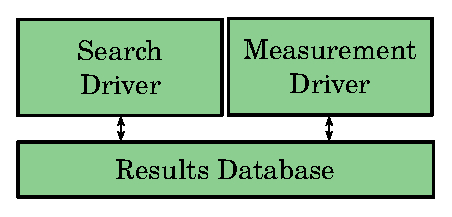
\includegraphics[scale=.75]{opentuner-implementation}
    \caption{Simplified OpenTuner Architecture.}
    \label{fig:ot-imp}
\end{figure}

Figure~\ref{fig:ot-imp} shows a high-level view OpenTuner's architecture.
Measurement and searching are done in separate modules, that share results
through the database. The search module requests measurements by registering
configurations to the database. The measurement module reads those
configurations and writes back the desired results. Currently, the
measurements are performed sequentially.

OpenTuner implements optimization techniques such as the
Nelder-Mead~\cite{nelder1965simplex} simplex
method and Simulated Annealing~\cite{kirkpatrick1983optimization}.
OpenTuner implements a resource sharing mechanism that aims to take
advantage of the strengths of each technique. A meta-technique
must balance the exploitation of a technique that has produced
good results in the past and the exploration of new, and possibly
best, techniques.

\section{Objectives} \label{sec:obj}

The objectives of this research project are the following

The remaining of this section describes each objective in detail,
and reports the current state of the research.

\subsection{Measurement Server and Client}

It's all about \texttt{\footnotesize process\_all}. Just checking.

\begin{figure}[htpb]
    \centering
    \begin{subfigure}{.45\textwidth}
        \centering
        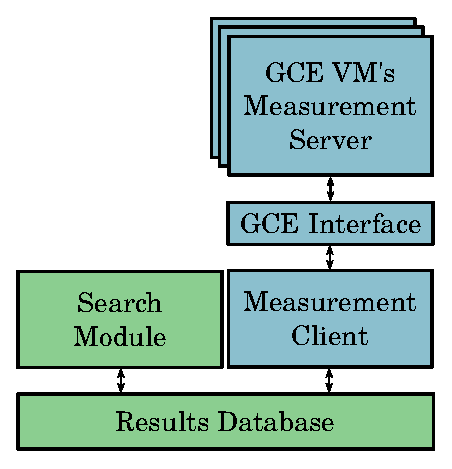
\includegraphics[scale=.75]{high-level-implementation}
        \caption{}
        \label{fig:high-level}
    \end{subfigure}%
    \begin{subfigure}{.45\textwidth}
        \centering
        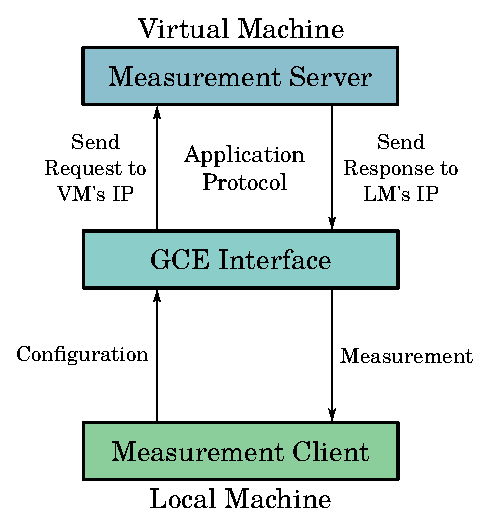
\includegraphics[scale=.75]{low-level-implementation}
        \caption{}
        \label{fig:low-level}
    \end{subfigure}%
\end{figure}

\begin{listing}[htpb]
    \begin{minted}[fontsize=\scriptsize]{python}
class MeasurementClient(MeasurementDriver):
    """
    Reads DesiredResults and requests VMs
    in the cloud to compute Results.
    """
    def __init__(self,
           measurement_interface,
           input_manager,
           **kwargs):
        super(MeasurementDriver, self).__init__(**kwargs)
        """
        Now, the client will instantiate and 
        configure the VM Measurement Servers.
        """

    def process_all(self):
        """
        Process all results in the
        database, by sending requests to
        VMs in the cloud and waiting
        responses.
        """
    \end{minted}
    \caption{A simple echo server in Python.}
    \label{fig:measurement-client}
\end{listing}


\subsection{Using the Google Compute Engine} \label{sec:pwork}

Development on the interface with Google Compute Engine
has already started, and the implementations are
available\footnote{All code is hosted at GitHub: \\
\texttt{\scriptsize github.com/phrb/measurement-server} \\
\texttt{\scriptsize github.com/phrb/autotuning-gce}}
under the GNU General Public License.

\begin{listing}[htpb]
    \begin{minted}[fontsize=\scriptsize]{python}
#!/usr/bin/env python

import socket

TCP_IP = ''
TCP_PORT = 8080
BUFFER_SIZE = 1024

s = socket.socket(socket.AF_INET, socket.SOCK_STREAM)
s.bind((TCP_IP, TCP_PORT))
s.listen(1)

conn, addr = s.accept()

while 1:
    data = conn.recv(BUFFER_SIZE)
    if not data: break
    conn.send(data)
    \end{minted}
    \caption{A simple echo server in Python.}
    \label{fig:server-test-code}
\end{listing}


\section{Experiments} \label{sec:exp}

\section{Research Schedule} \label{sec:sched}

\section{Conclusion} \label{sec:conclusion}

\bibliographystyle{plainnat}
\bibliography{ref}

\end{document}
